\documentclass[journal, a4paper]{IEEEtran}

% some very useful LaTeX packages include:

%\usepackage{cite}      % Written by Donald Arseneau
                        % V1.6 and later of IEEEtran pre-defines the format
                        % of the cite.sty package \cite{} output to follow
                        % that of IEEE. Loading the cite package will
                        % result in citation numbers being automatically
                        % sorted and properly "ranged". i.e.,
                        % [1], [9], [2], [7], [5], [6]
                        % (without using cite.sty)
                        % will become:
                        % [1], [2], [5]--[7], [9] (using cite.sty)
                        % cite.sty's \cite will automatically add leading
                        % space, if needed. Use cite.sty's noadjust option
                        % (cite.sty V3.8 and later) if you want to turn this
                        % off. cite.sty is already installed on most LaTeX
                        % systems. The latest version can be obtained at:
                        % http://www.ctan.org/tex-archive/macros/latex/contrib/supported/cite/

\usepackage{graphicx}   % Written by David Carlisle and Sebastian Rahtz
                        % Required if you want graphics, photos, etc.
                        % graphicx.sty is already installed on most LaTeX
                        % systems. The latest version and documentation can
                        % be obtained at:
                        % http://www.ctan.org/tex-archive/macros/latex/required/graphics/
                        % Another good source of documentation is "Using
                        % Imported Graphics in LaTeX2e" by Keith Reckdahl
                        % which can be found as esplatex.ps and epslatex.pdf
                        % at: http://www.ctan.org/tex-archive/info/

%\usepackage{psfrag}    % Written by Craig Barratt, Michael C. Grant,
                        % and David Carlisle
                        % This package allows you to substitute LaTeX
                        % commands for text in imported EPS graphic files.
                        % In this way, LaTeX symbols can be placed into
                        % graphics that have been generated by other
                        % applications. You must use latex->dvips->ps2pdf
                        % workflow (not direct pdf output from pdflatex) if
                        % you wish to use this capability because it works
                        % via some PostScript tricks. Alternatively, the
                        % graphics could be processed as separate files via
                        % psfrag and dvips, then converted to PDF for
                        % inclusion in the main file which uses pdflatex.
                        % Docs are in "The PSfrag System" by Michael C. Grant
                        % and David Carlisle. There is also some information
                        % about using psfrag in "Using Imported Graphics in
                        % LaTeX2e" by Keith Reckdahl which documents the
                        % graphicx package (see above). The psfrag package
                        % and documentation can be obtained at:
                        % http://www.ctan.org/tex-archive/macros/latex/contrib/supported/psfrag/

%\usepackage{subfigure} % Written by Steven Douglas Cochran
                        % This package makes it easy to put subfigures
                        % in your figures. i.e., "figure 1a and 1b"
                        % Docs are in "Using Imported Graphics in LaTeX2e"
                        % by Keith Reckdahl which also documents the graphicx
                        % package (see above). subfigure.sty is already
                        % installed on most LaTeX systems. The latest version
                        % and documentation can be obtained at:
                        % http://www.ctan.org/tex-archive/macros/latex/contrib/supported/subfigure/

\usepackage{url}        % Written by Donald Arseneau
                        % Provides better support for handling and breaking
                        % URLs. url.sty is already installed on most LaTeX
                        % systems. The latest version can be obtained at:
                        % http://www.ctan.org/tex-archive/macros/latex/contrib/other/misc/
                        % Read the url.sty source comments for usage information.

%\usepackage{stfloats}  % Written by Sigitas Tolusis
                        % Gives LaTeX2e the ability to do double column
                        % floats at the bottom of the page as well as the top.
                        % (e.g., "\begin{figure*}[!b]" is not normally
                        % possible in LaTeX2e). This is an invasive package
                        % which rewrites many portions of the LaTeX2e output
                        % routines. It may not work with other packages that
                        % modify the LaTeX2e output routine and/or with other
                        % versions of LaTeX. The latest version and
                        % documentation can be obtained at:
                        % http://www.ctan.org/tex-archive/macros/latex/contrib/supported/sttools/
                        % Documentation is contained in the stfloats.sty
                        % comments as well as in the presfull.pdf file.
                        % Do not use the stfloats baselinefloat ability as
                        % IEEE does not allow \baselineskip to stretch.
                        % Authors submitting work to the IEEE should note
                        % that IEEE rarely uses double column equations and
                        % that authors should try to avoid such use.
                        % Do not be tempted to use the cuted.sty or
                        % midfloat.sty package (by the same author) as IEEE
                        % does not format its papers in such ways.

\usepackage{amsmath}    % From the American Mathematical Society
                        % A popular package that provides many helpful commands
                        % for dealing with mathematics. Note that the AMSmath
                        % package sets \interdisplaylinepenalty to 10000 thus
                        % preventing page breaks from occurring within multiline
                        % equations. Use:
%\interdisplaylinepenalty=2500
                        % after loading amsmath to restore such page breaks
                        % as IEEEtran.cls normally does. amsmath.sty is already
                        % installed on most LaTeX systems. The latest version
                        % and documentation can be obtained at:
                        % http://www.ctan.org/tex-archive/macros/latex/required/amslatex/math/



% Other popular packages for formatting tables and equations include:

%\usepackage{array}
% Frank Mittelbach's and David Carlisle's array.sty which improves the
% LaTeX2e array and tabular environments to provide better appearances and
% additional user controls. array.sty is already installed on most systems.
% The latest version and documentation can be obtained at:
% http://www.ctan.org/tex-archive/macros/latex/required/tools/

% V1.6 of IEEEtran contains the IEEEeqnarray family of commands that can
% be used to generate multiline equations as well as matrices, tables, etc.

% Also of notable interest:
% Scott Pakin's eqparbox package for creating (automatically sized) equal
% width boxes. Available:
% http://www.ctan.org/tex-archive/macros/latex/contrib/supported/eqparbox/

% *** Do not adjust lengths that control margins, column widths, etc. ***
% *** Do not use packages that alter fonts (such as pslatex).         ***
% There should be no need to do such things with IEEEtran.cls V1.6 and later.

\usepackage[utf8]{inputenc}
\usepackage[czech]{babel}

\usepackage{xcolor}
\usepackage{listings}
\lstset{basicstyle=\ttfamily,
showstringspaces=false,
commentstyle=\color{red},
keywordstyle=\color{blue}
}

\usepackage{amsmath}

% Your document starts here!
\begin{document}

% Define document title and author
\title{Dětská chůvička s adaptabilním ovládáním hlasitosti}
\author{Jan Cach\\
Faculty of Informatics and Management\\
University of Hradec Kralove,\\
Hradec Kralove, Czech Republic\\
jan.cach@uhk.cz
}

	\maketitle

% Write abstract here
\begin{abstract}
	Tato práce se zabývá využitím jednodeskového počítače, např. Raspberry Pi a mobilní aplikace pro účely monitoringu dětského spánku. Mini počítač je využit jako zvukový server, který zaznamenává zvuk z mikrofonu a odesílá ho po místní síti do mobilní aplikace k dalšímu zpracování. Mobilní aplikace zpracuje přijatý zvuk, který je následně přehrán na mobilním zařízení. V průběhu zpracování zvuku aplikace rozhoduje o hladině hlasitosti zvuku přijatého ze zvukového serveru a upravuje automaticky hlasitost telefonu tak, aby uživatel co nejlépe slyšel co se děje v místnosti, kde je snímán zvuk. Aplikace nahrazuje dětskou chůvičku a nejčastěji ji využijí rodiče malých dětí.
\end{abstract}

\textbf{
\textit{
Keywords - adaptivní ovládání hlasitosti, Raspberry Pi, Android, dětská chůvička 
}
}
% Each section begins with a \section{title} command

% uvod
\section{INTRODUCTION/ÚVOD}
Další oblastí, kde můžeme mini počítač využít je pro sledování miminek a dětí během spánku. Malé děti a novorozenci stráví spánkem jednu třetinu až jednu polovinu svého života. Spánek těchto dětí není pravidelný a dochází k jejich náhodnému probouzení \cite{childsleep}. Dětská chůvička na monitorování dětí je nápomocná v případech, kdy se novorozeně nachází v jiné místnosti než rodiče. Rodiče díky tomu vědí jak jejich dítě spí a nemusejí nutně být s dítětem v jedné místnosti po celou dobu co dítě spí a zároveň vědí co se s jejich potomkem děje. \par
V této práci bude pro vytvoření dětské chůvičky využit mini počítač Raspberry Pi. Raspberry Pi je jednodeskový mini počítač, který byl původně určen pro výuku základů informatiky a programování. Jeho popularita se postupně rozšířila i mimo školu a díky malé velikosti, rozšiřitelnosti o různé moduly a malé energetické náročnosti se stal jedním z lídru na poli zařízení pro internet věcí \cite{raspberryweb}. \par
Mini počítače nedosahují výkonu stolních počítačů. Z tohoto důvodu je potřeba použít optimalizovaný operační systém, který nevyčerpá všechny systémové zdroje a mini počítač tak bude moci provozovat další aplikace. Pro platformu Raspberry Pi je dostupný oficiální operační systém pojmenovaný Raspbian. Tento operační systém je optimalizovaný pro Raspberry Pi, je založen na linuxové distribuci Debian. Ve svém základu obsahuje nástroje pro správu systému a programování \cite{raspbian}. \par
Pro vytvoření prototypu bude využit výše zmíněný mini počítač společně s připojeným či zabudovaným mikrofonem. Tento počítač s připojeným mikrofonem bude sloužit jako hudební server. Na takovýto hudební server bude možné se připojit pomocí aplikace v telefonu. \par
Aplikace bude s hudebním serverem komunikovat prostřednictvím síťového připojení. Využití aplikace není jednostranné a může být využito např. jako dětská chůvička, odposlechové zařízení, k poslechu hudby nebo může být využito k jednoduché komunikaci. Aplikace by měla nabízet snadné a přehledné ovládání. Základní funkcionalita aplikace bude spočívat v přehrávání zvuků přenesených z hudebního serveru. Aplikace bude dále nabízet adaptivní ovládaní hlasitosti. Adaptivní ovládání hlasitosti telefonu bude automaticky přizpůsobovat hlasitost telefonu tak, že při příliš malé hladině hlasitosti z přijímacího zařízení zesílí výstup mobilního telefonu a naopak zeslabí výstup telefonu při vysoké hladině hlasitosti přijaté z vysílacího zařízení. \par
Aplikace bude vyvíjena pro operační systém Android v programovacím jazyce Java s využitím příslušných knihoven pro Android platformu. Jako vývojové prostředí bude použito Android Studio, které nabízí mnoho nástrojů pro tvorbu kódu, grafického rozhraní, ladění a debugování programů bez nutnosti vlastnit telefon s operačním systémem android \cite{androidstudio}.

% problem definition
\section{PROBLEM DEFINITION/DEFINICE PROBLÉMU}
V obchodě pro mobilní telefony s operačním systémem Android Play Store je dostupných několik aplikací pro sledování dětí. Tyto aplikace mohou být rozděleny podle způsobu jakým upozorňují na probuzení dítěte. První kategorie aplikací, pokud detekuje zvýšený hluk, zašle SMS zprávu s upozorněním na předem zadané číslo, případně začne na toto číslo volat. Druhý typ aplikací využívá pro upozornění bezdrátovou síť WiFi případně dostupnou mobilní síť. Výhodou tohoto řešení je šetření nákladů za posílání SMS či volání a také možnost přenášet i video. \par
Do porovnání byly vybrány aplikace se stejným zaměřením a podobnými funkcemi. Sledovanými aspekty u konkurenčních aplikací jsou ovladatelnost a přehlednost aplikace, jak aplikace pracuje se zvukem a možnost připojení více poslechových zařízení. \par
První aplikací je Dormi. Aplikace Dormi pracuje na principu jednoho vysílacího zařízení s možností připojení více odposlouchávacích zařízení přes domácí síť. Aplikace má funkci inteligentní audio, která nastavuje snímání intenzity zvuku tak, aby rodičům neunikl žádný zvuk, který jejich dítě vydává. Ovládání aplikace je přehledné a vzhledu není co vytknout. Nevýhodou může být brána nutnost použití jednoho telefonu jako zařízení pro snímání zvuku. Pro používání aplikace bez omezení je nutné zakoupit plnou verzi aplikace. Jedinou nevýhodu aplikace je nutnost manuálně měnit hlasitost telefonu pro lepší slyšitelnost zvuku. \par
Další aplikace nese název Wifi Baby Monitor funguje na stejném principu jako Dormi. Jeden telefon je použitý pro snímání zvuku a další se mohou na tento telefon připojit a přehrávat zvuk ze zdroje. Vzhled aplikace je jednoduchý, až zastaralý. Aplikace ukazuje informace jako teplota, vlhkost stav baterie a čas sledování, které získává ze zařízení, které zvuk přehrává. Tyto informace jsou však na obrazovce rozmístěny chaoticky a nemají příliš velkou přidanou hodnotu. Aplikace nabízí automatickou kalibraci mikrofonu. Ovšem během testování tato funkce nefungovala dvou různých zařízeních. Další nevýhodou je nutnost manuálně nastavovat hlasitost telefonu pro lepší slyšitelnost zvuku, stejně jako tomu bylo u aplikace Dormi. \par
Třetí a poslední testovanou aplikací byla aplikace Nancy Baby Monitor. Aplikace má velice povedený vzhled, ale na telefonu s menším displejem logo překrývalo funkci nastavení citlivosti mikrofonu, tudíž nebylo možné citlivost měnit. Aplikace dále umožňuje uložení spárovaného telefonu, takže není potřeba pokaždé zadávat pin pro spárování. Stejně jako je tomu u dvou předchozích aplikací i u aplikace Nancy Baby Monitor musíme hlasitost telefonu měnit manuálně pokud chceme lépe slyšet např. plačící dítě. \par
Ze srovnání a testování vybraných aplikací bylo zjištěno, že žádná z aplikací nesplňuje všechny požadavky. Všechny testované aplikace umožňovaly připojení více zařízení pro poslech. Aplikace Nancy Baby Monitor jako jediná podporovala uložení aktuálního nastavení, které zjednodušší dlouhodobé používání aplikace tím, že není potřeba při každém spuštění znovu zadávat nastavení pro připojení. Všechny aplikace nabízely možnost upravit citlivost mikrofonu, při které je spuštěno upozornění na probuzení dítěte. Ovšem ve všech případech se jednalo o manuální nastavování.
Aplikace bude vytvořena pro platformu Android s funkcemi jako je přenášení zvuku od dítěte do telefonu a automaticky upravovat hlasitost telefonu tak, aby případný pláč a další zvuky, byly dobře slyšitelné. Aplikace také nabídne možnost uložení daného nastavení pro opětovné použití.

% new solution

\section{NEW SOLUTION/NOVÉ ŘEŠENÍ}
Z porovnání konkurenčních řešení v předchozí kapitole byly definovány požadavky na aplikaci. V této kapitole bude popsáno jak budou jednotlivé problémy vyřešeny. \par
Prvním problémem bude samotné zaznamenávání zvuku a jeho následný přenos do mobilního telefonu k dalšímu zpracování. V tomto směru bude aplikace fungovat na odlišném principu. Nebudou použity dva mobilní telefony jako u konkurenčních aplikací, ale minipočítač s připojeným mikrofonem a jeden mobilní telefon s aplikací na příjem zvuku. Pro tento účel bude využit zvukový server nazývaný Pulse Audio. Tento hudební server nabízí například slučování více zvuků do jednoho, nebo možnost přenášet zvuk po síti, detailní popis funkčnosti je uveden v \cite{pulseaudio}. A právě k přenášení zvuků po síťi bude Pulse Audio server využit. Server bude tuto službu nabízet na ip adrese a specifickém portu. Mikrofon snímá vibrace ve vzduchu a převádí je na elektrické signály. Později mohou být tyto zvukové signály vyhodnoceny jako hodnota signálu funkce času nebo přepočet do frekvenční domény. \par
    Dalším úkolem je zpracování přenášeného zvuku v telefonu. Bude potřeba vyřešit jak přehrát přijímaný zvuk v RAW formátu a jak s ním dále pracovat. Tento formát obsahuje pouze zvuková data a neobsahuje žádné další informace jako jsou vzorkovací frekvence, bitová hloubka nebo počet kanálů. Kritickým bodem je převedení dat v RAW formátu na měřitelnou jednotku se kterou se dá dále pracovat. Cílovou jednotkou je běžně používaná $dB_{SPL}$ , neboli hladina akustického zvuku. Tato problematika je zpravována v  \cite{dbspl} Takto získaná data bude možné porovnávat, pracovat s nimi a také je vhodně zobrazovat. \par
    Z předchozího odstavce známe jednotku, konkrétně decibel (dB), která nám umožňuje provádět další analýzu nad zvukovými daty. Konkrétně nás bude zajímat jak je vysoká hladina zvuku, který přijímáme ze vzdáleného zvukového serveru. Aplikace bude automaticky upravovat zvuk telefonu v závislosti na úrovni hlasitosti zvuku ze zvukového serveru. Algoritmus se bude vždy snažit nabídnout takovou hladinu zvuku, která bude posluchači příjemná, zdroj zvuku bude srozumitelný, čímž posluchači odpadne nutnost manuálně měnit zvuk telefonu. Nízka hladina zvuku na straně zvukového serveru znamená v našem kontextu, že sledované dítě spí nevydává žádné zvuky. Další hladinou mohou být střední hlasitost na straně zvukového serveru. V tomto případě se například dítě probudilo, otáčí se v posteli hraje si s nějakou hračkou. Nejvyšší hladina hlasitosti na straně serveru indikuje, že dítě se probudilo a brečí. Rozsah jednotlivých hladin byl stanoven s využitím tabulky \ref{tab:table1}. Tabulka byla vypracována s využitím zdroje \cite{tableres}. 

\begin{table}[h!]
    \begin{center}
        \caption{Klasifikace hladiny zvuku}
        \label{tab:table1}
        \begin{tabular}{l|c}
            \textbf{Zdroj zvuku} & \textbf{Hladina v dB}\\
            \hline
            Dýchaní & 10\\
            Šepot, šustění listí & 20\\
            Klidná venkovská oblast & 30\\
            Knihovna, městské okolí & 40\\
            Tiché předměstí, domácí rozhovor & 50\\
            Hluk kanceláře, hudba na pozadí & 60\\
            Rádio, televize, vysavac & 70\\
        \end{tabular}
        \end{center}
\end{table}

    Nejnižší rozmezí úrovně hlasitosti je 0 - 22 dB. Tento rozsah je brán jako klidový interval, kdy dítě spí. Jestliže přijímaný zvuk spadá do tohoto intervalu, je potřebné mít hlasitost nastavenou na nejvyšší úroveň. Zvuk telefonu bude tedy nastaven na hodnotu 95 % maximální hlasitosti telefonu. Další úrovní bude úroveň hlasitosti, která bude v intervalu od 23 - 45 dB. Jak bylo uvedeno výše, toto rozmezí hladiny zvuku může znamenat, že dítě se probudilo, ale nebrečí. V takovém případě je hlasitost telefonu nastavena na 65 %. Další interval, kdy dítě brečí a jedná se tak o nejsilnější možný zaznamenaný zvuk je daný intervalem 46 - 60 dB. Pokud se úroveň snímaného zvuku bude nacházet v daném intervalu hlasitost telefonu bude nastavena na 40 %. Jestliže bude úroveň zvuku přijatého ze zvukového serveru větší než 60 dB, bude hlasitost telefonu snížena na 10 % procent pro příjemný poslech. \par
    Posledním úkolem bude vhodně prezentovat zvuková data pomocí dostupných komponent jako jsou zvuková stupnice nebo grafy. Aplikace by tedy měla nabídnout informace o aktuální hlasitosti telefonu a také o hladině zvuku snímaném na vzdáleném zvukovém serveru.



% implementace
\section{IMPLEMENTATION/IMPLEMENTACE ŘEŠENÍ}
V předchozí kapitole byly představeny jednotlivé přístupy ke každé části vytvářené aplikace. V této kapitole bude ukázáno jak jsou jednotlivé části implementovány. \par
Jak bylo uvedeno v předchozí kapitole jako zvukový server pro přenos zvuku bude použit PulseAudio sound server. Tento zvukový server je možné nastavit pomocí grafického rozhraní nebo příkazy. Následující skript ukazuje nastavení serveru pomocí příkazů zadaných přes terminál. 
{\small
\begin{lstlisting}[language=bash,caption={bash code}]
#!/bin/sh
case "$1" in start)
$0 stop 
pactl load-module module-simple-protocol-tcp 
rate=48000 format=s16le channels=2 source=0 
record=true port=8000

pactl load-module module-loopback
;;
stop)
pactl unload-module `pactl list | 
grep tcp -B1 | grep M | sed 's/[^0-9]//g'`
pactl unload-module module-loopback
;;
*)
echo "Usage: $0 start|stop" >&2
;;
esac
\end{lstlisting}
}
Nejdříve je načten modul tcp pro sdílení zvuku po síťi. Ke správnému fungování musíme ještě předat modulu správné parametry. Prvním parametrem je rate, který značí vzorkovací frekvenci, dále format označuje vzorkovací formát. Channels s hodnotou 2 zde značí stereo. Pro označení zdroje zvuku je použit parametr source a v skriptu označuje zvukovou kartu, která přehrává veškerý zvuk. Znamená to tedy, že veškerý zvuk, který má být přehrán je odeslán po síti. Dalším parametrem je sítový port na který se bude možné z telefonu připojit pro získání zvuku. Posledním volitelným parametrem je auth-ip. Tento parameter definuje jaké ip adresy, případně jaký rozsah ip adres, se může na zvukový server připojit. Jedná se tedy o bezpečnostní prvek, který omezuje přístup pouze pro specifické uživatele. Druhý příkaz pactl load-module loopback module říká, že zvuk z mikrofonu je poslán na zvukovou kartu k přehrání a díky tomu je odeslán po síťi na přijímající zařízení. Příkazy pactl unload-module slouží pro řádné ukončení zvukového serveru. Jak pracovat s PulseAudio serverem je vysvětleno v \cite{manpages}. \par
V následujících odstavcích bude představena implementace aplikace. Jak je uvedeno výše aplikace bude vytvořena pro platformu Android. Důvodu pro zvolení této platformy je více, z nichž ty nejzásadnější jsou široká rozšířenost a dostupnost tohoto systému. Aplikace bude dostupná i pro starší verze systému Android. Konkrétně pro verze 4.3 a vyšší. Podle \cite{androidstudio} tak bude aplikace fungovat přibližně na 95 \% zařízeních se systémem Android. \par
Strukturu aplikace můžeme rozdělit na dvě základní části. První část je uživatelské rozhraní a definice chování k jednotlivým prvkům na obrazovkách aplikace. Např. jaká akce má být vykonána, jestliže uživatel klikl na tlačítko nebo inicioval návrat na předchozí obrazovku. Ve druhé části aplikace se nacházejí podpůrné třídy, které implementují logickou část aplikace. Sem se řadí např. Třída, která má na starost ukládání a načítání nastavení nebo třída, která přehrává zvuk, který získá ze vzdáleného hudebního serveru. Dále se podíváme na jednotlivé části aplikace podrobněji. \par
Mezi triviální třídy patří aktivita WelcomeActivity, která pouze zobrazuje logo a název aplikace po dobu čtyř vteřin. Následně je uživatel přesměrován na menu aplikace, reprezentován třídou MenuActivity, které slouží jako rozcestník pro přechod na další aktivity. Dále to jsou aktivity ServerSettingsActivity, která zobrazuje návod jak nastavit zvukový server, a aktivita AboutAppActivity, která pouze zobrazuje základní informace o uživateli. \par
Nastavení aplikace obstarává aktivita SettingsActivty. Tato aktivita obsahuje čtyři textová pole pro zadání jednotlivých parametrů, jako je ip adresa zvukového serveru a port, dále vzorkovací frekvence a výběr počtu kanálů mono nebo stereo. Pro ukládání a načítání nastavení je využita třída SettingsManager. Tato třída má jednu veřejnou metodu pro ukládání, které se pouze předají parametry a třída provede uložení. Při ukládání umí tato třída ověřit zda byla zadána platná ip adresa a také port. Pokud ověření selže je uživateli zobrazena hláška o špatně zadaném parametru a uložení se neprovede. Data jsou ukládána ve formátu JSON. Při startu aplikace se automaticky načte uložené nastavení, pokud existuje. Tento krok uživateli urychluje práci pokud používá stejné nastavení. \par
Hlavní aktivitou aplikace je ListenActivity. Z této aktivity je možné přehrávat zvuky ze vzdáleného serveru a sledovat hlasitost telefonu a také hladinu zvuku na straně serveru. Rozložení jednotlivých komponent aplikace je uvedeno na obrázku \ref{fig:listenactivity}.


V horní části obrazovky se nachází aktuální hlasitost telefonu, reprezentovaná číselně v procentech a také pomocí progress baru. Poté následují informace o zdroji zvuku. Konkrétně hladina hlasitosti pro zdrojový zvuk v decibelech společně s grafem, který zobrazuje vývoj hladiny v čase. Pro implementaci grafu je použita knihovna Android GraphView \cite{graphview}. S pomocí této knihovny je možné zobrazit vývoj hladiny zvuku zdroje v čase, který se aktualizuje každou vteřinu a zobrazuje data v reálném čase. Přehrávání zvuku se spustí tlačítkem playMusic a k tomuto účelu využívá třídu PlaySound. Třída PlaySound je spuštěna ve vlastním vlákně tak, aby bylo možné interagovat s UI aplikace během přehrávání zvuku. Přehrávání je implementováno metodou run. V této metodě nejdříve dojde k vytvoření Socketu, který reprezentuje síťové spojení na zvukový server. Dále je zde třída AudioTrack, která zajištuje samotné přehrání zvuku. Třídě jsou předána data, která jsou získána ze socketu, a AudioTrack třída zajistí jejich přehrání na telefonu. \par
Pro analýzu zvuku je potřebné z přijatého zvuku vypočítat jeho hladinu. Pro tento účel je vytvořena třída SoundManager. Podle experimentu provedeného zde \cite{stackoverflow}, byl pro výpočet decibelu sestaven následující vzorec. \par

\begin{equation*}
	s = 20log( \frac{0.00002+\frac{0.6325-0.00002}{32767}m\\}{0.00002})\\ 	
\end{equation*} 

Nejvyšší naměřená hodnota, kterou mikrofon naměří je 90 dB neboli 0.6325 Pa. Hodnota 0.00002 je referenční minimum. Mikrofon vrací hodnoty jako Java typ short v rozmezí hodnot -32768 až 32767, který je normalizován jako absolutní hodnota, odtud tedy hodnota 32767. Hodnota value ve vzorci představuje aktuální hodnotu, kterou mikrofon vrátil a jedná se o proměnnou v daném vzorci. Výsledkem je hladina zvuku v decibelech. Tato hodnota je dále použita pro výpočet klouzavého průměru velikosti hladiny zvuku. Klouzavý průměr je počítán z pěti předchozích hodnot a pomáhá redukovat náhlé výstřelky hodnot. Výsledné změny hladiny zvuku jsou tak plynulejší než kdyby se brala v potaz pouze aktuální hodnota hladiny zvuku. Hodnota získaná z klouzavého průměru je dále použita pro nastavení hlasitosti v telefonu. Změny hlasitosti probíhají podle definovaných pravidel v předchozí kapitole. Pro nastavení hlasitosti je potřebné znát maximální hlasitost telefonu, která se liší v závislosti na modelu telefonu. Toto zajišťuje metoda returnVolumeLevel. Metoda si za pomoci třídy AudioManager zjistí maximální hlasitost daného stroje a vrátí hlasitost pro zadaná procenta. Posledním krokem je aktualizace UI komponent aktuálními hodnotami, kterou provede funkce updateUI.

\begin{figure}[h]
	 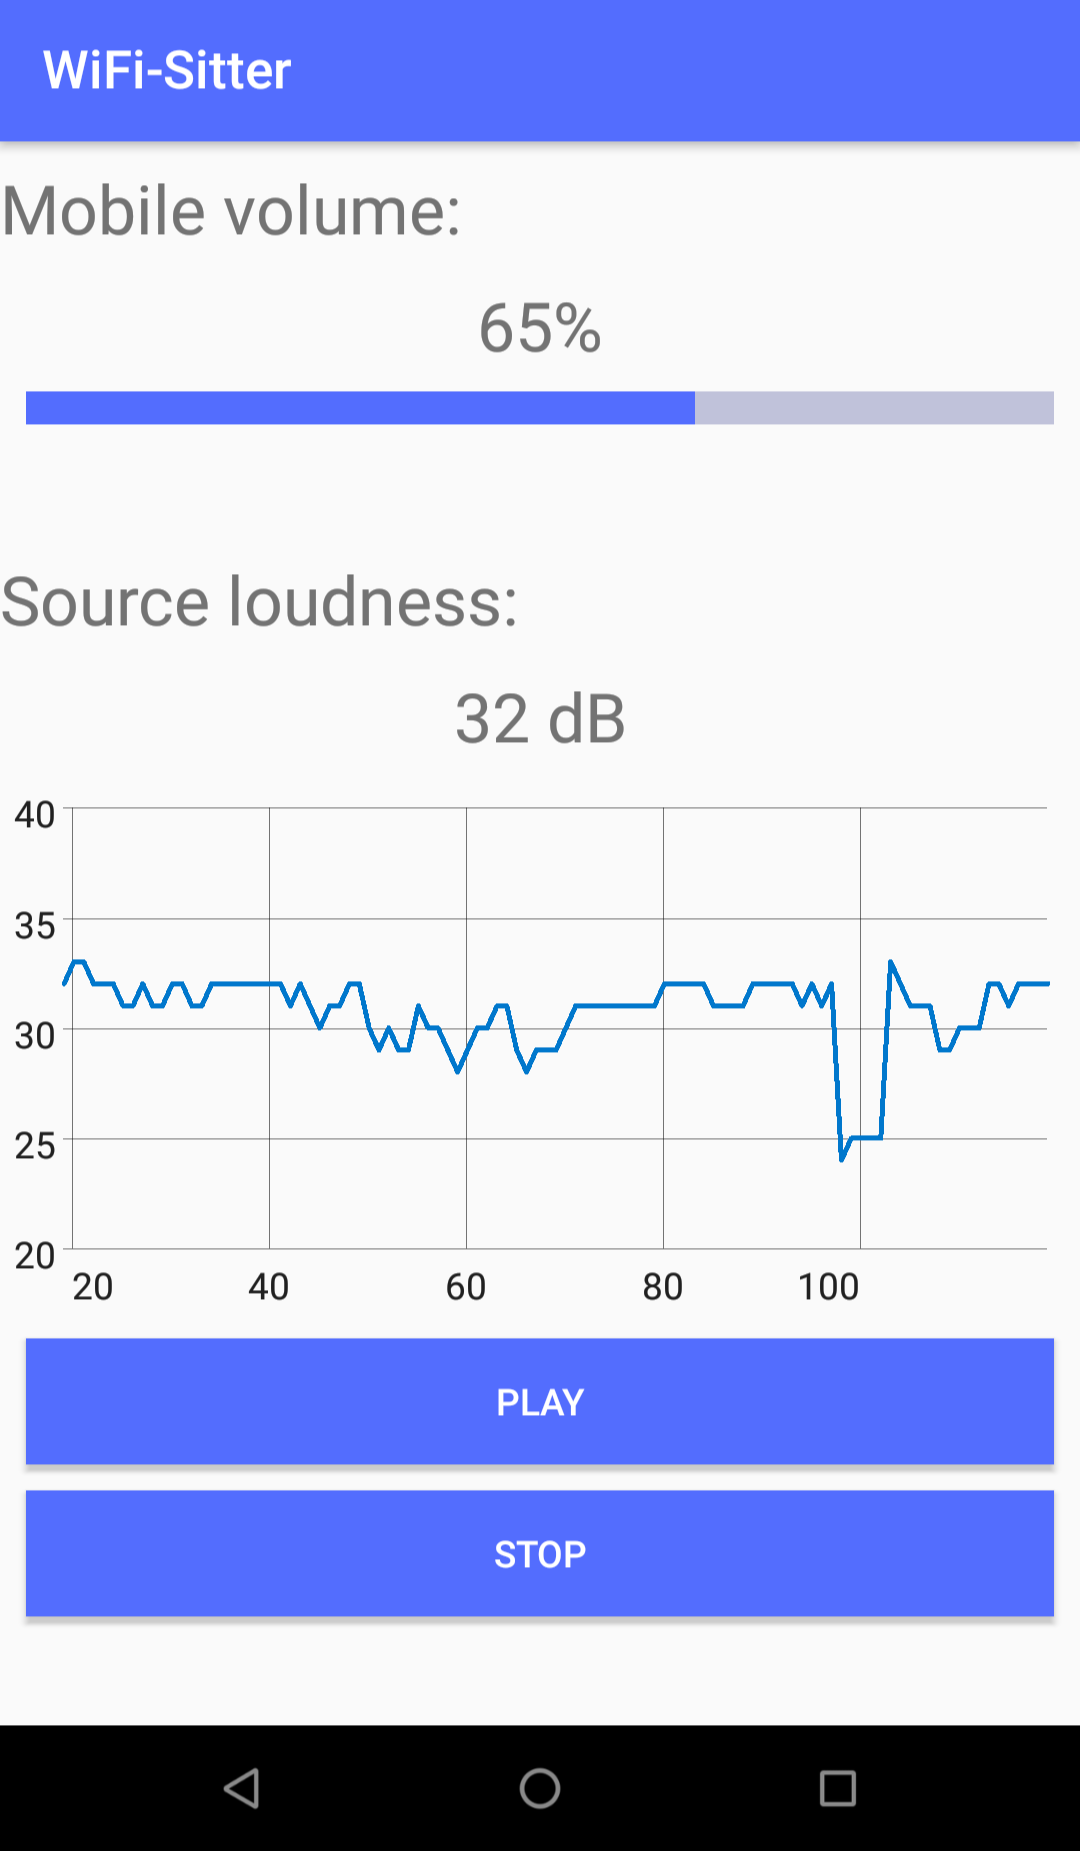
\includegraphics[width=\linewidth,scale=0.2]{obrazovka.png}
	 \caption{Liste activity}
	 \label{fig:listenactivity}
\end{figure}

\section{TESTING OF DEVELOPED APPLICATION/TESTOVÁNÍ VYVINUTÉ APLIKACE}
Testování aplikace bylo rozděleno na dvě části, kde v každé části byla testována odlišná část aplikace. V první části bylo testováno nastavení hudebního serveru uživateli s rozdílnými počítačovými zkušenostmi. Ve druhé části bylo poté testování fungování aplikace na různých zařízeních. \par
Cílem prvního testu je zjistit jak náročné je spuštění hudebního serveru pro snímání zvuku. Test byl proveden na dvou osobách, rozdílných počítačových dovedností. První osoba, pracující v oblasti IT, dokázala bez větších problémů zprovoznit hudební server podle návodu v mobilní aplikaci. Druhá osoba, běžný uživatel počítače, již tak úspěšný nebyl. Největším problémem bylo samotné ovládání linuxového operačního systému a použití terminálu pro nastavení hudebního serveru. V tomto případě, by bylo dobré vytvořit video, které by do nejmenšího detailu popsalo jednotlivé kroky tak, aby i uživatel, který nemá skušenosti s linuxovým operačním systémem byl schopný zapnout a nastavit hudební server.\par 
Druhá část testování měla za úkol otestovat aplikaci na různých zařízeních. Aplikace byla testování na třech rozdílných mobilních telefonech. Prvním v testu byl telefon Samsung Galaxy Xcover 3 s operačním systémem Android verze 6. Vzhled a rozložení komponen bylo na telefonu v pořádku. Stejně tak dopadlo i ukládání a načítání uloženého nastavení. Během přehrávání aplikace občas docházelo k výpadku zvuku a bylo nutné aplikaci restartovat. Během přehrávání, po uplynutí zhruba 1 minuty, začlo docházet  ke zpožďování zvuku, které se ustálilo přibližně na 3 vteřinách. Dalším telefonem byl mobilní telefon LG Nexus 5x s verzí Androidu 7. Ovládání aplikace fungovalo na tomto telefonu dobře, včetně ukládání a načítání nastavení. Stejně jako u předchozího telefonu i u Nexusu docházelo ke zpožďování zvuku. Posledním testovaným telefonem byl Goodle Pixel XL s nejnověší verzí Andoidu 8. Na Pixelu aplikace fungovala obdobně jako na Nexusu. Rozložení komponent a interakce fungovaly podle očekávání. Adaptabilní ovládání hlasitosti fungovalo na všech zařízeních dobře. Hlasitost telefonu se automaticky měnila podle nastavených hladin.Problémem bylo pouze zpoždění zvuku na testovaných telefonech.

% conclusion
\section{CONCLUSION/ZÁVĚR}
Cílem této práce bylo vytvořit aplikaci na monitorování děstského spánku s využitím jednodeskového počítače pro záznam zvuku a mobilní aplikace pro přehrání zvuku. Aplikace měla být rozšířena o automatické ovládání hlasitosti telefonu v závislosti na velikosti hladiny zvuku na straně zvukového serveru. Po prostudování existujících řešení byli stanoveny jednotlivé požadavky na aplikaci. Aplikace byla následně vytvořena tak, aby splnila všechny požadavky. Zvukový server může být spuštěn na Raspberry Pi počítačích, či na domácím laptopu s operačním systémem linux a využitím externího či zabudovaného mikrofonu. Aplikace pro příjem zvuku byla naprogramována pro většinu mobilních telefonů s operačním systémem android. \par
Aplikace si jistě najde své příznivce v řadách rodičů. Tato aplikace nabízí vlastnit plnohodnotnou dětskou chůvičku zdarma bez nutnosti kupovat drahé zařízení. Další výhodou může být například další využití této aplikace ke sdílení hudby po domácí síťi do více mobilních zařízení. Řešení tedy není vázáno pouze na jeden mobilní telefon, ale může být připojeno několik mobilních telefonů naráz. \par
Aplikace obsahuje všechny definované funkce, ale jsou zde další funkce, které by aplikaci vylepšily. Nápady jak zlepšit aplikaci může být například přidání přenosu videa do telefonu nebo možnost přehrát zvuk z telefonu na zvukovém serveru např. pro utišení dítěte. Další oblastí, která by se dala zlepšit je design aplikace, který by uživatelům nabídl přehlednějsí a jednodušší ovládání. Z testování také vyplynulo, že běžní uživatelé mají problém s nastavením hudebního serveru. Řešením může být vytvoření detailního popisu, jak krok za krokem nastavit hudební server. Napříkad pomocí videa nebo obrázkového návodu.

% Now we need a bibliography:
\begin{thebibliography}{10}

	\bibitem{raspberry1}
	LECCESE, Fabio, Marco CAGNETTI, Stefano DI PASQUALE, Sabino GIARNETTI a Maurizio CACIOTTA. A New Power Quality Instrument Based on Raspberry-Pi. Electronics [online]. 2016, 5(4), 64- [cit. 2018-04-26]. DOI: 10.3390/electronics5040064. ISSN 2079-9292. Dostupné z: \url{http://www.mdpi.com/2079-9292/5/4/64}
\newline

	\bibitem{raspberry2}
	BERNABÉ, Gregorio, Raúl HERNÁNDEZ a Manuel E. ACACIO. Parallel implementations of the 3D fast wavelet transform on a Raspberry Pi 2 cluster. The Journal of Supercomputing [online]. 2018, 74(4), 1765-1778 [cit. 2018-04-26]. DOI: 10.1007/s11227-016-1933-2. ISSN 0920-8542. Dostupné z: \url{http://link.springer.com/10.1007/s11227-016-1933-2}
\newline

	\bibitem{raspberry3}
	SIANTIKOS, Georgios, Theodoros GIANNAKOPOULOS a Stasinos KONSTANTOPOULOS. Monitoring Activities of Daily Living Using Audio Analysis and a RaspberryPI: A Use Case on Bathroom Activity Monitoring. RÖCKER, Carsten, John O'DONOGHUE, Martina ZIEFLE, Markus HELFERT a William MOLLOY, ed. Information and Communication Technologies for Ageing Well and e-Health [online]. Cham: Springer International Publishing, 2017, 2017-07-20, s. 20-32 [cit. 2018-04-26]. Communications in Computer and Information Science. DOI: 10.1007/978-3-319-62704-5-2. ISBN 978-3-319-62703-8. Dostupné z: \url{http://link.springer.com/10.1007/978-3-319-62704-5-2}
\newline

	\bibitem{childsleep}
		RAMOS, Kathleen D. a Davin M. YOUNGCLARKE. Parenting Advice Books About Child Sleep: Cosleeping and Crying It Out. Sleep [online]. 2006, 29(12), 1616-1623 [cit. 2018-04-26]. DOI: 10.1093/sleep/29.12.1616. ISSN 1550-9109. Dostupné z: \url{https://academic.oup.com/sleep/article-lookup/doi/10.1093/sleep/29.12.1616}
\newline	

	\bibitem{raspberryweb}
		Raspberry Pi - Teach, Learn, and Make with Raspberry Pi [online]. United Kingdom [cit. 2018-04-26]. Dostupné z: url{https://www.raspberrypi.org/}
\newline

	\bibitem{raspbian}
		\textit{Raspbian} [online]. [cit. 2018-04-26]. Dostupné z: \url{https://www.raspbian.org/}


\newline

	\bibitem{androidstudio}
		\textit{Android Studio} [online]. Mountain View: Google [cit. 2018-04-26]. Dostupné z: \url{https://developer.android.com/studio/}
\newline

	\bibitem{pulseaudio}
		\textit{PulseAudio} [online]. 2017 [cit. 2018-04-28]. Dostupné z: \url{https://www.freedesktop.org/wiki/Software/PulseAudio/}
\newline

	\bibitem{dbspl}
		ZAMORA, Willian, Carlos T. CALAFATE, Juan-Carlos CANO a Pietro MANZONI. Smartphone tuning for accurate ambient noise assessment. In: Proceedings of the 15th International Conference on Advances in Mobile Computing & Multimedia - MoMM2017 [online]. New York, New York, USA: ACM Press, 2017, 2017, s. 115-122 [cit. 2018-04-28]. DOI: 10.1145/3151848.3151854. ISBN 9781450353007. Dostupné z: \url{http://dl.acm.org/citation.cfm?doid=3151848.3151854}
\newline

	\bibitem{tableres}
		Comparitive Examples of Noise Levels. \textit{The IAC Mission | Industrial Noise Control} [online]. NORTH AURORA, Illinois, 2018 [cit. 2018-04-28]. Dostupné z: \url{http://www.industrialnoisecontrol.com/comparative-noise-examples.htm}
\newline

	\bibitem{manpages}
		Pactl(1) - Linux man page. \textit{Die.net} [online]. 2017 [cit. 2018-04-29]. Dostupné z: \url{https://linux.die.net/man/1/pactl}
\newline

	\bibitem{androidstudio}
		AndroidStudio. \textit{Android Developers} [online]. 2018 [cit. 2018net-04-29]. Dostupné z: \url{https://developer.android.com/studio/}
\newline

	\bibitem{graphview}
	\textit{Android Graph View} [online]. Jonas Gehring, 2018 [cit. 2018-04-29]. Dostupné z: \url{http://www.android-graphview.org/}
\newline

	\bibitem{stackoverflow}
		Lukas Ruge. What does Android’s getMaxAmplitude() function for the
		MediaRecorder actually give me? - Stack Overflow. URL: \url{http://stackoverflow.com/a/14870458/1119508}

\end{thebibliography}

% Your document ends here!
\end{document}
